\documentclass[aspectratio=169,17pt]{beamer}
\usepackage[ngerman]{babel}
\usepackage{fontspec}
\setmainfont{Arial}
\setsansfont{Arial}
\usepackage{newtxmath}
\renewcommand{\familydefault}{\sfdefault}
\renewcommand{\rmdefault}{\sfdefault}
\usepackage{amsmath,amssymb}
\usepackage{booktabs}
\usepackage{colortbl}
\usepackage{graphicx}
\usepackage{tikz}
\usetikzlibrary{positioning}
\newcommand{\QFinal}{877.8}
\newcommand{\QFinalFull}{877.781}
\newcommand{\KDurchfluss}{9.646}
\newcommand{\QDry}{578.8}
\newcommand{\QChiller}{299.0}
\newcommand{\PElectric}{74.2}
\newcommand{\EElectric}{650.1}
\newcommand{\PChiller}{59.805}
\newcommand{\PFans}{14.064}
\newcommand{\PPumps}{0.338}
\newcommand{\EnergyCostFinal}{116.36}
\newcommand{\MaintenanceFinal}{21.58}
\newcommand{\QCondenser}{358.8}
\newcommand{\QAirRejection}{952.0}
\newcommand{\QFloodStress}{12.48}
\newcommand{\BufferVolume}{8280}
\newcommand{\PipeDiameter}{0.70}
\newcommand{\QReserve}{1053.3}
\newcommand{\QModule}{175.6}
\newcommand{\QStorage}{0.0303}
\newcommand{\EvapRate}{358.3}
\newcommand{\EvapAnnual}{11.30}
\newcommand{\EvapFraction}{15.6}
\newcommand{\DilutionFlow}{52.3}
\newcommand{\DilutionRatio}{22.8}
\newcommand{\PassiveArea}{4.4}
\newcommand{\CapexFinal}{719}
\newcommand{\OpexFinal}{137.9}
\newcommand{\NpvHybrid}{2.90}
\newcommand{\NpvUpfront}{3.01}
\newcommand{\NpvSaving}{112}
\newcommand{\NpvEvap}{0.78}
\newcommand{\NpvDilution}{11.48}
\newcommand{\FailureMinutes}{23}
\newcommand{\PoolTau}{3.02}
\newcommand{\QSampleLow}{480}
\newcommand{\QSampleHigh}{1528}
\newcommand{\NpvSampleLow}{2.36}
\newcommand{\NpvSampleHigh}{3.81}


\definecolor{navy}{HTML}{102A3D}
\definecolor{blue}{HTML}{176B87}
\definecolor{orange}{HTML}{D97732}
\definecolor{soft}{HTML}{EAF2F5}
\definecolor{gray}{HTML}{64707A}
\definecolor{green}{HTML}{3D7A57}

\setbeamertemplate{navigation symbols}{}
\setbeamertemplate{footline}{}
\setbeamercolor{normal text}{fg=navy,bg=white}
\setbeamercolor{frametitle}{fg=navy,bg=white}
\setbeamerfont{frametitle}{size=\fontsize{26}{31},series=\bfseries}
\setbeamerfont{normal text}{size=\fontsize{17}{21}}
\setbeamersize{text margin left=8mm,text margin right=8mm}

\newcommand{\slidefoot}[1]{\vfill{\fontsize{10.5}{13}\selectfont\color{gray}#1\par}}
\newcommand{\bignumber}[2]{{\fontsize{34}{38}\selectfont\bfseries\color{blue}#1\par}\vspace{1mm}{\fontsize{14}{17}\selectfont\color{gray}#2\par}}
\newcommand{\compactnumber}[2]{{\fontsize{26}{30}\selectfont\bfseries\color{blue}#1\par}\vspace{1mm}{\fontsize{12.5}{15}\selectfont\color{gray}#2\par}}
\newcommand{\source}[1]{{\fontsize{10.5}{13}\selectfont\color{gray}#1\par}}

\begin{document}

\begin{frame}[plain]
  \vspace{13mm}
  {\fontsize{42}{47}\selectfont\bfseries 878 Megawatt\par}
  \vspace{6mm}
  {\fontsize{22}{27}\selectfont Dauerhafte Kühlung für das Blautopf-Szenario\par}
  \vfill
  {\fontsize{14}{18}\selectfont PlaNeT SimTech, Science Slam\par}
  {\fontsize{12}{15}\selectfont Team-ID TEST-K31pro-max, 07.11.2026\par}
\end{frame}

\begin{frame}{Ein Kelvin entscheidet}
  \vspace{2mm}
  \begin{columns}[T]
    \column{0.52\textwidth}
      \bignumber{9,646 MW}{Wärmeabfuhr pro Kelvin beim mittleren Quellstrom}
      \vspace{3mm}
      \begin{equation*}
        \dot Q=\rho\,\dot V\,c_p\,\Delta T
      \end{equation*}
    \column{0.43\textwidth}
      \bignumber{877,8 MW}{für 91 K im zehnten Prognosejahr}
      \vspace{2mm}
      {\fontsize{14}{17}\selectfont Das Szenario erwärmt das Tiefenwasser von 9 auf 100 °C. Der Entwurf kühlt den gesamten betroffenen Strom zurück auf 9 °C.\par}
  \end{columns}
  \slidefoot{Quellen und Rechnung [2,4], konservativer Vollstromfall.}
\end{frame}

\begin{frame}{Zwei Kontrollvolumen}
  \begin{columns}[T]
    \column{0.63\textwidth}
      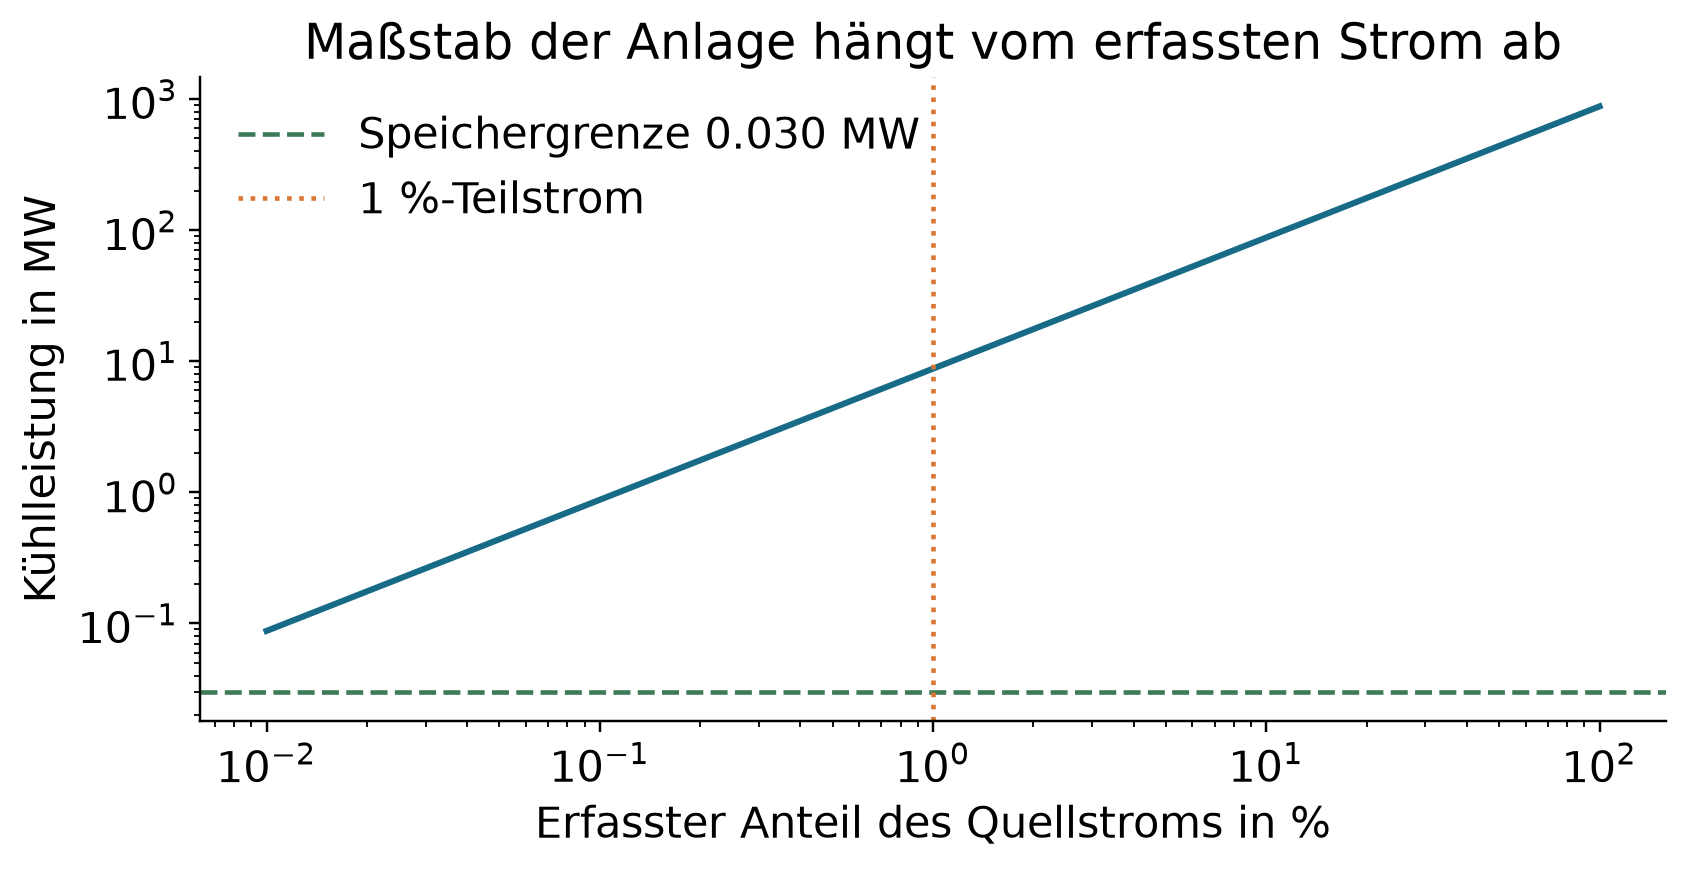
\includegraphics[width=\textwidth,height=36mm,keepaspectratio]{../report/figures/fig06_teilstrom.png}
    \column{0.33\textwidth}
      \bignumber{29.000-fach}{Verhältnis von Vollstrom zu isolierter Speicherrechnung}
      \vspace{1mm}
      {\fontsize{12}{15}\selectfont Vollstrom 877,8 MW, Speicher 0,0303 MW. Ein 1-\%-Teilstrom senkt die Last auf 8,8 MW.\par}
  \end{columns}
  \slidefoot{Eigene Rechnung mit Python und Kimi K3.1 Pro, Volumenannahme 25.000 m³.}
\end{frame}

\begin{frame}{Sieben physikalische Wege}
  \renewcommand{\arraystretch}{1.0}
  {\fontsize{11.5}{14}\selectfont
  \begin{tabular}{@{}p{11mm}p{90mm}p{35mm}@{}}
    \toprule
    Weg & Entscheidender Befund & Urteil \\
    \midrule
    \rowcolor{soft} H1 & Trockene Hybridkühlung schließt die Wärmebilanz & Referenz \\
    H2 & Verdunstung verbraucht 11,3 Mio. m³/a & ökologisch schlechter \\
    H3 & Kaltwasserbedarf 52,3 m³/s & keine Quelle belegt \\
    H4 & Karsteingriff braucht unbekannte Fließwege & Forschungsoption \\
    H5 & Bypass lässt das Becken weiter heiß & unzureichend \\
    H6 & Druck verschiebt nur den Siedepunkt & abgelehnt \\
    H7 & Passive Fläche 4,39 km² bei Sommerluft & unzureichend \\
    \bottomrule
  \end{tabular}\par}
  \slidefoot{Alternativenvergleich unter identischer Last, Berechnungen in \texttt{results.json}.}
\end{frame}

\begin{frame}{Die zweistufige Kühlung}
  \centering
  \resizebox{\textwidth}{!}{%
  \begin{tikzpicture}[
    stage/.style={draw=navy,rounded corners=1mm,align=center,minimum height=20mm,text width=35mm,font=\fontsize{15}{18}\selectfont},
    flow/.style={-{latex},very thick,blue},
    heat/.style={-{latex},very thick,orange}]
    \node[stage] (source) {Tiefenwasser\\100 °C};
    \node[stage,right=12mm of source] (dry) {Trockenkühler\\100 auf 40 °C\\578,8 MW};
    \node[stage,right=12mm of dry] (chiller) {Kältemaschine\\40 auf 9 °C\\299,0 MW};
    \node[stage,right=12mm of chiller] (buffer) {Puffer\\8280 m³\\Rampe 91 h};
    \node[stage,above=15mm of dry,text width=46mm] (air) {Luft als externe Wärmesenke\\952,0 MW};
    \draw[flow] (source) -- (dry);
    \draw[flow] (dry) -- (chiller);
    \draw[flow] (chiller) -- (buffer);
    \draw[heat] (dry.north) -- (air.south);
    \draw[heat] (chiller.north) -- (air.south);
  \end{tikzpicture}}
  \vspace{1mm}

  {\fontsize{12.5}{15}\selectfont Sechs Stränge in jeder Ausbaustufe, fünf im Betrieb und einer in Reserve. Jedes aktive Endmodul kühlt 0,46 m³/s.\par}
  \slidefoot{Wärmebilanz einschließlich Kondensator- und Hilfsenergie [8], eigene Anlagenskizze.}
\end{frame}

\begin{frame}{Bei Ausfall zählen Minuten}
  \begin{columns}[T]
    \column{0.40\textwidth}
      \bignumber{23 min}{bis 20 °C nach vollständigem Kühlungsausfall im zehnten Jahr}
      \vspace{2mm}
      {\fontsize{12.5}{15}\selectfont Interne Alarmschwelle, keine behördliche Blau-Grenze und keine Siedezeit.\par}
    \column{0.55\textwidth}
      {\fontsize{13.5}{16}\selectfont
      \begin{itemize}
        \item sechs Stränge mit N+1-Reserve in jeder Ausbaustufe
        \item zwei Netzeinspeisungen und 48 Stunden Notstromreserve
        \item unabhängige Temperatur- und Druckmessung
        \item Sollwert rampe am Kälteauslass, 91-h-Stresstest
      \end{itemize}\par}
  \end{columns}
  \slidefoot{Beckenvolumen 25.000 m³ als Rechenannahme, Zeitkonstante 3,02 h.}
\end{frame}

\begin{frame}{Der Preis des trockenen Weges}
  \begin{columns}[T]
    \column{0.62\textwidth}
      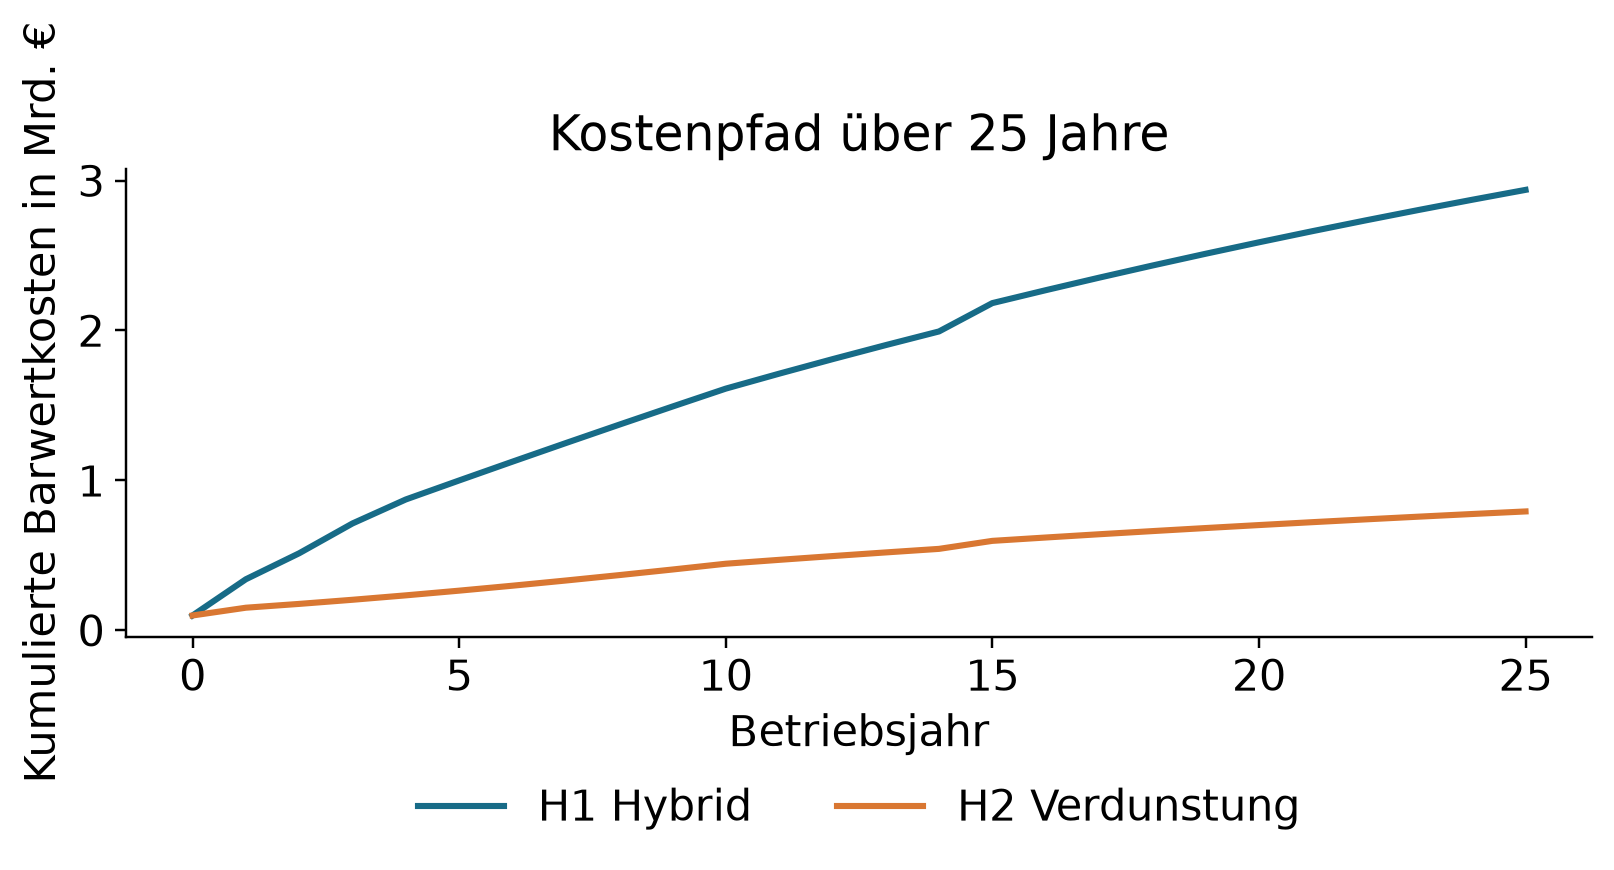
\includegraphics[width=\textwidth,height=44mm,keepaspectratio]{../report/figures/fig03_kostenpfad.png}
    \column{0.34\textwidth}
      \compactnumber{722 Mio. €}{Investition mit Reserve}
      \vspace{1mm}
      \compactnumber{2,94 Mrd. €}{Barwert über 25 Jahre}
      \vspace{1mm}
      {\fontsize{12}{15}\selectfont Verdunstung: 0,79 Mrd. €, 11,3 Mio. m³/a Wasser. H1: 193,0 kt CO$_2$/a mehr Stromemissionen [23].\par}
  \end{columns}
  \slidefoot{Szenario-Schätzungen in Euro von 2026, keine Angebote [13,16,18,19].}
\end{frame}

\begin{frame}{Die Hülle begrenzt das Versprechen}
  \begin{columns}[T]
    \column{0.64\textwidth}
      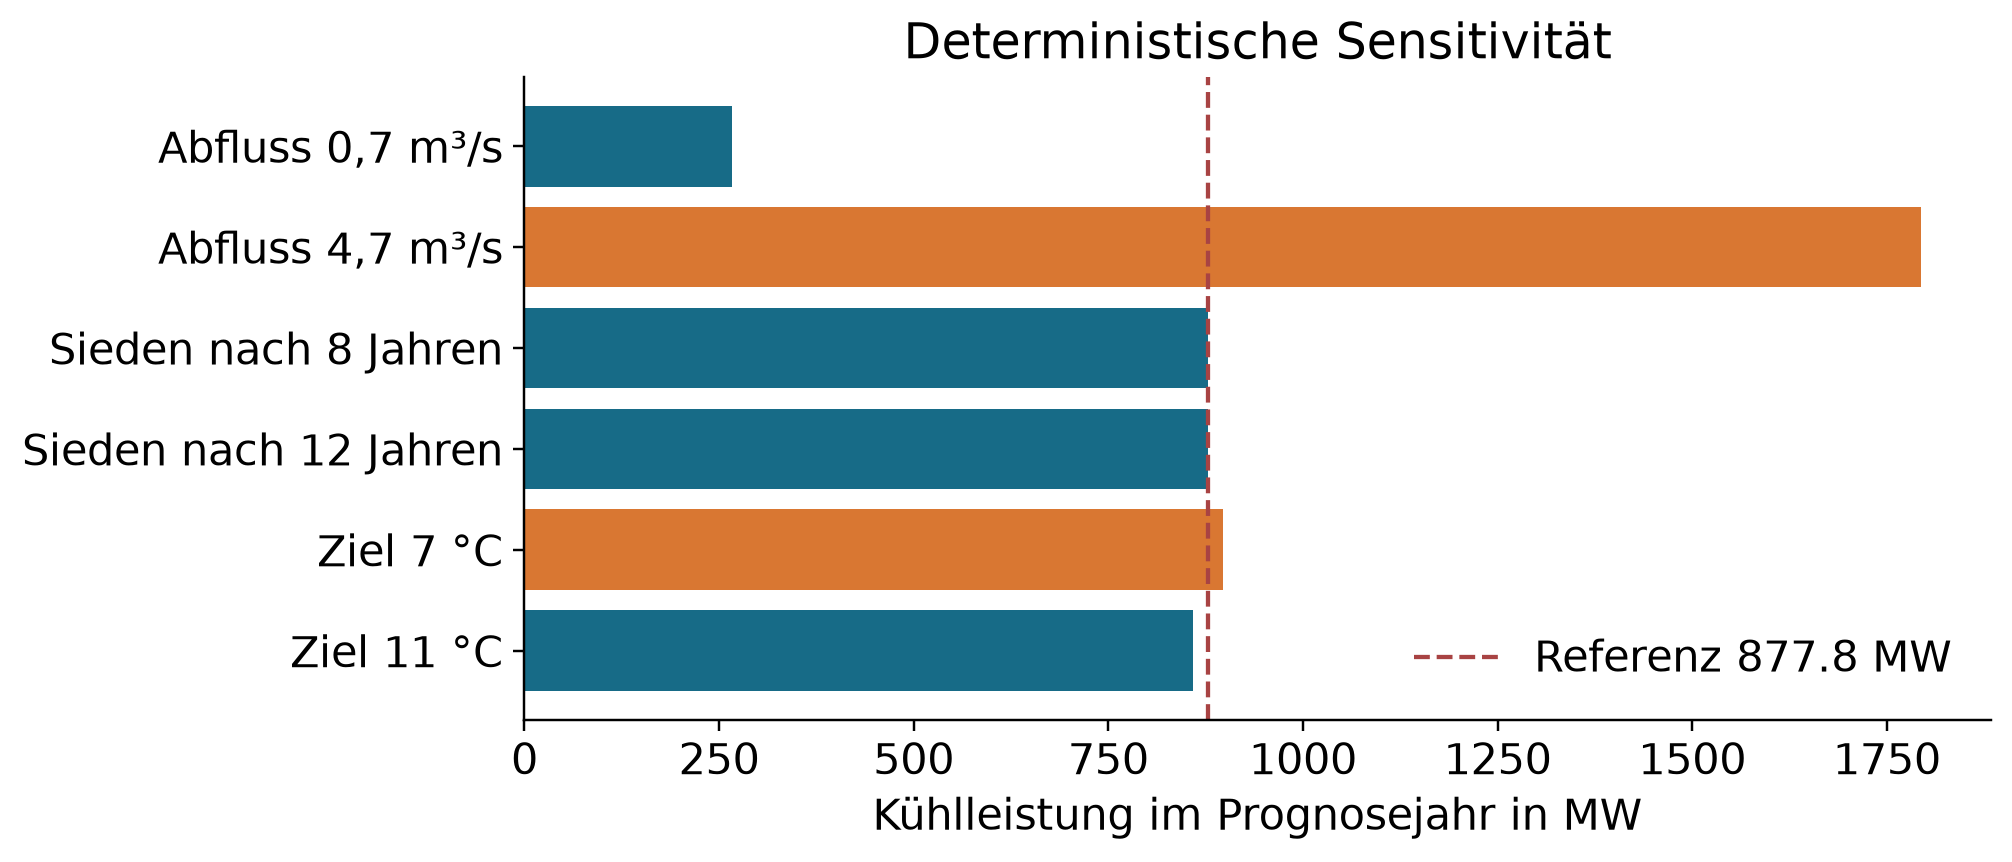
\includegraphics[width=\textwidth,height=32mm,keepaspectratio]{../report/figures/fig04_sensitivitaet.png}
    \column{0.32\textwidth}
      \compactnumber{12,48 GW}{Hochwasser-Stresstest bei 32,7 m³/s}
      \vspace{1mm}
      {\fontsize{11.5}{14}\selectfont Nicht abgedeckt. Mehr Wärme erfordert einen neuen Entwurf.\par}
  \end{columns}
  \slidefoot{Varianten [2,3]. Referenz: höchstens 2,3 m³/s betroffener Strom.}
\end{frame}

\begin{frame}{Messung und Kühlentscheidung}
  \renewcommand{\arraystretch}{1.0}
  {\fontsize{12}{14.5}\selectfont
  \begin{tabular}{@{}p{70mm}p{69mm}@{}}
    \toprule
    Messung & Konsequenz \\
    \midrule
    Temperatur und Druck in beiden Karstästen & Ort und Verlauf der Anomalie \\
    Durchfluss und Tracer & betroffener Anteil des Quellstroms \\
    verteilte Temperatursonden & Tiefenprofile statt Oberflächenbild \\
    Kühlversuche & gemessene statt angenommene Leistung \\
    Energiezähler an der Luftseite & kein Wärmerückfluss ins Gewässer \\
    \bottomrule
  \end{tabular}\par}
  \slidefoot{Nur ein nachweisbar kleiner Teilstrom rechtfertigt eine kleine Anlage. Messprogramm [3,11,12].}
\end{frame}

\begin{frame}{Schlussfolgerung}
  \vspace{3mm}
  {\fontsize{22}{27}\selectfont\bfseries Die 878 MW folgen aus dem Vollstromszenario. Sie sind keine beliebig gewählte Anlagengröße.\par}
  \vspace{4mm}
  {\fontsize{15}{19}\selectfont Die Anlage hält 9 °C innerhalb ihrer belegten Hülle. Vor dem Bau entscheiden Tracer, Durchfluss und Tiefenmessung über den tatsächlichen Maßstab.\par}
  \vfill
  \source{Hauptquellen [2,3,4,8,9,13,16]. Vollständige Quellen im Bericht.}
  \source{KI-Offenlegung: Inhalt, Modell und Sprechtext mit Kimi K3.1 Pro bei maximaler Reasoning-Stufe. Recherche mit DeepSeek-V4.1-Flash. Vertonung mit eSpeak NG 1.52.0. Kein Live-Mitschnitt und keine menschliche Prüfung.}
\end{frame}

\end{document}
